%%%%%%%%%%%%%%%%%%%%%%% file typeinst.tex %%%%%%%%%%%%%%%%%%%%%%%%%
%
% This is the LaTeX source for the instructions to authors using
% the LaTeX document class 'llncs.cls' for contributions to
% the Lecture Notes in Computer Sciences series.
% http://www.springer.com/lncs       Springer Heidelberg 2006/05/04
%
% It may be used as a template for your own input - copy it
% to a new file with a new name and use it as the basis
% for your article.
%
% NB: the document class 'llncs' has its own and detailed documentation, see
% ftp://ftp.springer.de/data/pubftp/pub/tex/latex/llncs/latex2e/llncsdoc.pdf
%
%%%%%%%%%%%%%%%%%%%%%%%%%%%%%%%%%%%%%%%%%%%%%%%%%%%%%%%%%%%%%%%%%%%


\documentclass[runningheads,a4paper]{article}

\setcounter{tocdepth}{3}
\usepackage{graphicx}
% For citations
\usepackage{natbib}
\usepackage{amsmath,amsfonts,amscd,amssymb}
\usepackage{dsfont}
\renewcommand{\vec}[1]{\mathbf{#1}}
\usepackage{hyperref}
\DeclareMathOperator*{\argmax}{argmax}
\DeclareMathOperator*{\argmin}{argmin}
\DeclareMathOperator*{\Corr}{Corr}
\newcommand{\R}{\mathds{R}}
\usepackage{multicol}
\usepackage{multirow}
\usepackage{pbox}
\usepackage{url}
\urldef{\mailsa}\path|{felix.biessmann,|
\newcommand{\keywords}[1]{\par\addvspace\baselineskip
\noindent\keywordname\enspace\ignorespaces#1}
\usepackage{booktabs}
\usepackage{color}
\newcommand{\felix}[1]{\textcolor{blue}{#1}}

\begin{document}

 % start of an individual contribution

% first the title is needed
\title{Speeding up the manifesto project: Active learning strategies for efficient automated political annotations}

% a short form should be given in case it is too long for the running head
\title{Speeding up the manifesto project: \\ Active learning strategies for \\efficient automated political annotations}

% the name(s) of the author(s) follow(s) next
%
% NB: Chinese authors should write their first names(s) in front of
% their surnames. This ensures that the names appear correctly in
% the running heads and the author index.
%
\author{
Felix Biessmann\thanks{felix.biessmann@gmail.com},~ 
Philipp Schmidt\thanks{schmidtiphil@gmail.com}
%Andreas Grafberger\thanks{}
}
%
%\authorrunning{Active Learning for Political Annotations}}
% (feature abused for this document to repeat the title also on left hand pages)

% the affiliations are given next; don't give your e-mail address
% unless you accept that it will be published
%\institute{
%\mailsa\\
%\mailsb\\
%\mailsc\\
%\url{http://www.springer.com/lncs}}

%
% NB: a more complex sample for affiliations and the mapping to the
% corresponding authors can be found in the file "llncs.dem"
% (search for the string "\mainmatter" where a contribution starts).
% "llncs.dem" accompanies the document class "llncs.cls".
%

%\toctitle{}
%\tocauthor{}
\maketitle

\begin{abstract} 
The Manifestoproject Corpus is an exceptional data source for political education as it combines political texts with valuable annotations by human experts. However the amount of data human annotators can label is very limited compared to the ever increasing amount of political texts published in manifestos, news media and social networks. The discrepancy between labeling budget and data that needs to be labelled highlights the necessity of automated annotations by means of machine learning (ML). Taking into account label consistency across human experts, which is often not perfect and thus requires to collect at least three labels per data point, this discrepancy is even worse. 

When only a small fraction of the available data can be labelled in order to train an ML model, the priority of which samples should be labelled first is important: Some samples are easy to classify - those should not be labelled with high priority, as the classifier will not learn much from them. For these samples it is relatively safe to have them labelled automatically by an ML model without wasting the time of human annotators. Other data points are difficult for the ML model; when labels for those are obtained first, the model will reach its optimal classification performance faster. 

In this study we leverage this insight, known in the ML community as active learning. We present offline experiments on the manifesto corpus showing that active learning strategies significantly speed up training of ML models for manifesto code annotations. This shows the potential of ML methods as assistive technology for political science. To demonstrate the benefits of this approach we present an implementation of a web based active learning annotation system that can be readily used for speeding up the manifesto annotations as well as annotations of other political texts.
\end{abstract} 

\section{Introduction}
\label{sec:intro}
%
\felix{Some motivation and a gentle intro to active learning will go here.}

\section{Related Work}\label{sec:related}
Throughout the last years automated content analyses for political texts have been conducted on a variety of text data sources (parliament data \, blogs, tweets, news articles, party manifestos) with a variety of methods, including sentiment analysis, stylistic analyses, standard bag-of-word (BOW) text feature classifiers and more advanced natural language processing tools. For an overview we refer the reader to \cite{Grimmer2013,Kaal2014}. 

The work closest related to this study is using machine learning classification models to identify political affiliation or bias on political speeches or manifesto data. In \cite{Yu2008} the authors extracted BOW feature vectors and applied linear classifiers to predict political party affiliation of US congress speeches. Similar work in \cite{Hirst2014} uses data from the Canadian parliament and the European parliament. 
Other work has focused on developing largely unsupervised for predicting political bias. Two popular methods are WordFish \cite{Slapin08ascaling} and WordScores \cite{Laver2003}, or improved versions thereof, see e.g. \cite{Lowe09scalingpolicy}. These approaches have been very valuable for {\em a posteriori} analysis of historical data but they do not seem to be used as much for analyses of new data in a predictive analytics setting. 

Taken together, there is a large body of literature on automated analysis of political texts. Except for few exceptions most previous work has focused on binary classification or on assignment of a one dimensional policy position (often corresponding to left vs right). Data sets such as the manifesto project allow for more fine grained analyses of political bias. Models trained on such data can give valuable insights in political texts in a predictive setting see e.g. \cite{Merz2016,Biessmann16}. While data set as the manifesto project allow to train classifiers that can give more detailed insight into political bias, they also impose a significant effort on the annotators. 

The scope of the manifesto project limits the to be annotated texts to a feasible amount, 'just' the party manifestos. But one can imagine scenarios in which not all data can be fully annotated. One such scenario could be a tight deadline for an analysis right before elections: parties release their programs only shortly before the elections and often these texts are too long to read by one single person before the elections \cite{merz2017}. In addition to relying on experts to interpret these programs, it can be helpful to use models trained on previously annotated data to assess the policies proposed in the party programs. This can help to get a better overview of the policies especially when new parties enter the political stage, see e.g. \cite{bronline}. 
Another scenario in which the labelling budget is limited is if one wants to annotate texts from online media. It can be important in many settings to have an expert view on the political bias of a text. But high volume of content published by online media does not allow for an expert analysis of all texts. In this context, automated text analysis with models trained on the manifesto project data can be helpful. In an ideal scenario one could use a model to automatically label texts for which the model is relatively certain to be correct and only send data to annotation by human experts when the model is uncertain. This idea is the basis of the active learning scenario we are considering in this work. 

\section{Data Sets and Feature Extraction}\label{sec:data}
%

\subsection{Data}
Annotated political text data was obtained from all manifesto texts of parties in Germany made available through the Manifesto Project \cite{manifesto}. 
Each sentence or in some cases also parts of a sentences is annotated with one of 56 political labels. Examples of these labels are {\em pro/contra protectionism, decentralism, centralism, pro/contra welfare}; for a complete list and detailed explanations on how the annotators were instructed see \cite{leftright}. In total this resulted in 48148 political statements. In order to obtain training data that would lead to reliable predictions in the experiments we discarded categories that had less than 1000 observed labels, which resulted in the 17 labels listed in \autoref{tab:valid_labels}.

\begin{table}
\centering
\label{tab:valid_labels} 

\begin{tabular}{rlr}
\toprule
 cmp\_code &                   label &  counts \\
\midrule
      503 &        social justice + &    4086 \\
      411 &        infrastructure + &    3085 \\
      501 &      environmentalism + &    2775 \\
      303 &  gov-admin efficiency + &    2580 \\
      403 &     market regulation + &    2513 \\
      504 &               welfare + &    2418 \\
      201 &  freedom/human rights + &    2410 \\
      701 &                labour + &    2199 \\
      506 &             education + &    2064 \\
      202 &             democracy + &    1918 \\
      305 &   political authority + &    1590 \\
      107 &      internationalism + &    1574 \\
      408 &          economic goals &    1298 \\
      706 &   non economic groups + &    1224 \\
      606 &        social harmony + &    1137 \\
      502 &               culture + &    1130 \\
      605 &         law and order + &    1117 \\
\bottomrule
\end{tabular}
\caption{List of valid labels and Manifesto Project Codes above 1000 counts.}
\end{table}

The reason we needed to discard the less frequent labels was merely because in the experiments we subsampled the data heavily in order to simulate cases in which only very few sentences could be labeled. This required us to discard rare labels as those are very likely to not be observed at all when subsampling only around 10\% of the data. 

\subsection{Bag-of-Words Vectorization}\label{sec:bow-vectorization}
Strings of each semantic unit (quasi sentence) were tokenised and transformed into bag-of-word vectors as implemented in scikit-learn \cite{scikit-learn}. We used the standard \href{http://scikit-learn.org/stable/modules/generated/sklearn.feature_extraction.text.HashingVectorizer.html}{HashingVectorizer}. The text of each semantic unit is transformed into a vector $\vec{x}\in\mathds{R}^d$ where $d=10^{18}$ is the size of the dictionary (here: number of hash buckets); the $w$th entry of $\vec{x}$ contains the count of the $w$th feature. In previous experiments we have tried several options for vectorizing the texts, including term-frequency-inverse-document-frequency normalisation, n-gram patterns up to size $n=3$, several cutoffs for discarding too frequent and too infrequent words and also most standard natural language processing procedures such as stemming or lemmatization, for some of these experiments we refer to \cite{Biessmann16}. These experiments showed that rather modest preprocessing, lowercasing and bigrams, resulted in best generalization performance. Hence in the current experiments we only used lower casing and unigram features, which were only slightly worse than bigrams.

\section{Classification Model and Training Procedure}\label{sec:model}
Bag-of-words feature vectors were used to train a multinomial logistic regression model. Let $y\in\{1,2,\dots,K\}$ be the true  label, where $K$ is the total number of labels and $\vec{W}=[\vec{w}_1,\dots,\vec{w}_K]\in\R^{d\times K}$ is the concatenation of the weight vectors $\vec{w}_k$ associated with the $k$th party then 
\begin{eqnarray}\label{eq:logreg_multiclass}
p(y=k|\vec{x},\vec{W}) = &\frac{e^{z_k}}{\sum_{j=1}^K e^{z_j}} \qquad \textrm{with }  z_k=&\vec{w}_k^{\top}\vec{x} \\\nonumber
\end{eqnarray}
%
We estimated $\vec{W}$ using stochastic gradient descent with 5 epochs through the training data set. The optimization function was obtained by adding a penalization term to the negative log-likelihood of the multinomial logistic regression objective and the optimization hence found the $\vec{W}$ that minimized
\begin{equation}\label{eq:objective}
L(\vec{W}, \vec{x}, \gamma) = - \log{\frac{e^{z_k}}{\sum_{j=1}^K e^{z_j}}}+ \gamma \| \vec{W} \|_{F}
\end{equation}
Where $\|~\|_F$ denotes the Frobenius Norm and $\gamma$ is a regularization parameter controlling the complexity of the model. 
The regularization parameter was optimized on a log-scaled grid from $10^{-4,\dots,4}$. The performance of the model was optimized using the negative log likelihood, but we also report all other standard measures for each class, in particular 

\begin{itemize}
\item Accuracy $\frac{\text{correct classifications}}{\# samples}$
\item Precision $\frac{TP} {FP + TP}$
\item Recall $\frac{TP}{TP + FN}$
\item F1 score $2\times \frac{\text{Precision} \times \text{Recall}}{\text{Precision} + \text{Recall}}$
\end{itemize}

where \textit{TP} and \textit{FP} stands for true positives and false positives, respectively.


\subsection{Model Selection and Evaluation}\label{sec:crossvalidation}
For model evaluation we kept 10\% of the entire training data separate in all experiments. For model selection, or hyper parameter optimization we only considered the regularization parameter as described in \autoref{sec:model}. All other hyper parameters related to preprocessing the data were kept fixed based on previous experiments reported in \cite{Biessmann16}. This restriction was made to speed up the experiments, as each training run involved hyper parameter optimization, which comes at a significant computational cost. All hyperparameters were optimized using 2-fold cross validation on the training set. 

\subsection{Active Learning Strategies}\label{sec:active_learning_strategies}
We employed three different active learning strategies which we will briefly outline below, for a detailed review on the topic and various strategies we refer to \cite{2012Settles}. 

\paragraph{Random Baseline} In order to simulate the standard procedure for sampling that does not take into account the uncertainty of the classifier we used random sampling from the pool of to-be-labeled examples. 

\paragraph{Uncertainty Sampling}
Uncertainty sampling queries samples $\vec{x}_i$ for which a classifier's top prediction is least confident
\begin{align}\label{eq:uncertainty_sampling}
\vec{x}_i = \argmax_{i,k} \left(1- p(y=k|\vec{x}_i,\vec{W})\right)
\end{align}
This strategy only takes into account the top prediction and hence could loose information from less likely classes, according to the model. 

\paragraph{Entropy Sampling}
Entropy sampling queries samples $\vec{x}_i$ for which a classifier's prediction for all classes is least confident
\begin{align}\label{eq:entropy_sampling}
\vec{x}_i = \argmax_{i} \sum_k p(y=k|\vec{x}_i,\vec{W}) \log(p(y=k|\vec{x}_i,\vec{W}))
\end{align}
This variant takes into account predictions for all classes and intuitively speaking might pick up too much information from noisy predictions for unlikely classes. 

\paragraph{Margin Sampling}
Margin sampling queries samples $\vec{x}_i$ for which a classifier's prediction for the top two predicted classes is minimal
\begin{align}\label{eq:entropy_sampling}
\vec{x}_i = \argmin_{i} \left(p(y=k_1|\vec{x}_i,\vec{W}) - p(y=k_1|\vec{x}_i,\vec{W}) \right)
\end{align}
where $k_1,~k_2$ are the classes that are most likely and second most likely, respectively, under the current model. 
This variant is a compromise between the uncertainty sampling and the entropy sampling strategy.

\subsection{Offline Experiment Setting}
We used the above active learning strategies to simulate a scenario in which a limited budget of labelling resources is available and the task is to train a model as best as possible on this labelling budget. The model performance was measured on a separate held out test data set. The best performance of a given model class was measured by performing model selection and training on all of the training data and testing on the test set. The active learning strategies were then compared by performing model selection and training on only a fraction of the training data, in particular 1\%, 10\%, 20\%, \dots, 100\%. For each subsampling of the data we performed all four sampling strategies. Sampling was performed using the last model on all samples that were not yet labeled and the newly sampled data points were joined with the already sampled data points. This setting allowed to estimate with which fraction of the entire training data each respective strategy yielded the best model, relative to the model trained on all training data. In order to obtain robust results we ran each experiment 100 times, meaning 100 times training and testing using each sampling strategy for each of the considered fractions of the training data. 

\section{Results}

We first report some results of a model that was trained on the entire training data, in order to illustrate the performance of the best performing model under the given model class. This will the bar against the active learning experiments will be compared. Afterwards we present the results of the active learning experiments in which we compare the strategies listed in \autoref{sec:active_learning_strategies} with a random baseline. 

\subsection{Baseline Model}\label{sec:results_baseline}
Example results for a baseline model trained on half the available training data is shown in \autoref{tab:baseline_model_report}. On average an F1 score of 0.48 was obtained with a simple linear logistic regression model and unigram features. This is comparable to results previously obtained on the complete set of manifesto codes and a model trained with exhaustive model selection on all relevant model and preprocessing hyperparameters. Also the result is comparable with the accuracy obtained in previous similar experiments performed on the same data \cite{Merz2016}.
\begin{table}
\centering
\begin{tabular}{cccccc}
\toprule
&  manifesto code & precision  &  recall&  f1-score &  support\\
\midrule
&   107&  0.60& 0.48& 0.53&  774\\
&   201&  0.51& 0.55& 0.53& 1194\\
&   202&  0.63& 0.57& 0.60&  983\\
&   303&  0.35& 0.41& 0.38& 1251\\
&   305&  0.46& 0.59& 0.52&  783\\
&   403&  0.52& 0.48& 0.50& 1281\\
&   408&  0.34& 0.17& 0.23&  628\\
&   411&  0.39& 0.60& 0.47& 1535\\
&   501&  0.61& 0.55& 0.58& 1380\\
&   502&  0.65& 0.41& 0.50&  587\\
&   503&  0.46& 0.52& 0.49& 2083\\
&   504&  0.34& 0.56& 0.43& 1179\\
&   506&  0.63& 0.48& 0.54& 1026\\
&   605&  0.56& 0.44& 0.49&  576\\
&   606&  0.63& 0.27& 0.38&  561\\
&   701&  0.59& 0.39& 0.47& 1123\\
&   706&  0.45& 0.26& 0.33&  615\\
\bottomrule
& avg / total&  0.50& 0.48& 0.48&17559\\
\end{tabular}
\caption{Precision, recall, F1 score and number of instances per class. }
\label{tab:baseline_model_report} 
\end{table}


\subsection{Active Learning Results}
\label{sec:active_learning_results}
We ran 100 offline experiments on all data for all active learning strategies and plot the median and 5th/95th percentile of the accuracies obtained with the respective model trained on a given fraction of the training data in \autoref{fig:active_learning_curves}. The results demonstrate that active learning clearly achieves superior performance compared to random sampling. In the large majority of cases, active learning resulted in a model that was indistinguishable from the best model that could have been obtained when training on all available training data with less than 80\% of the total training data. Random sampling, the baseline strategy, required 100\% of the training data in order to achieve the same performance. 

We did not observe in our experiments a clear distinction between the different active learning strategies. This could be related to the fact that we discarded rare labels, which led to a rather small amount of classes. Hence the differences between the active learning strategies and their respective advantages for a large number of labels did not help as much as they would have with more labels and an even more skewed label distribution. 

\begin{figure}
\begin{center}
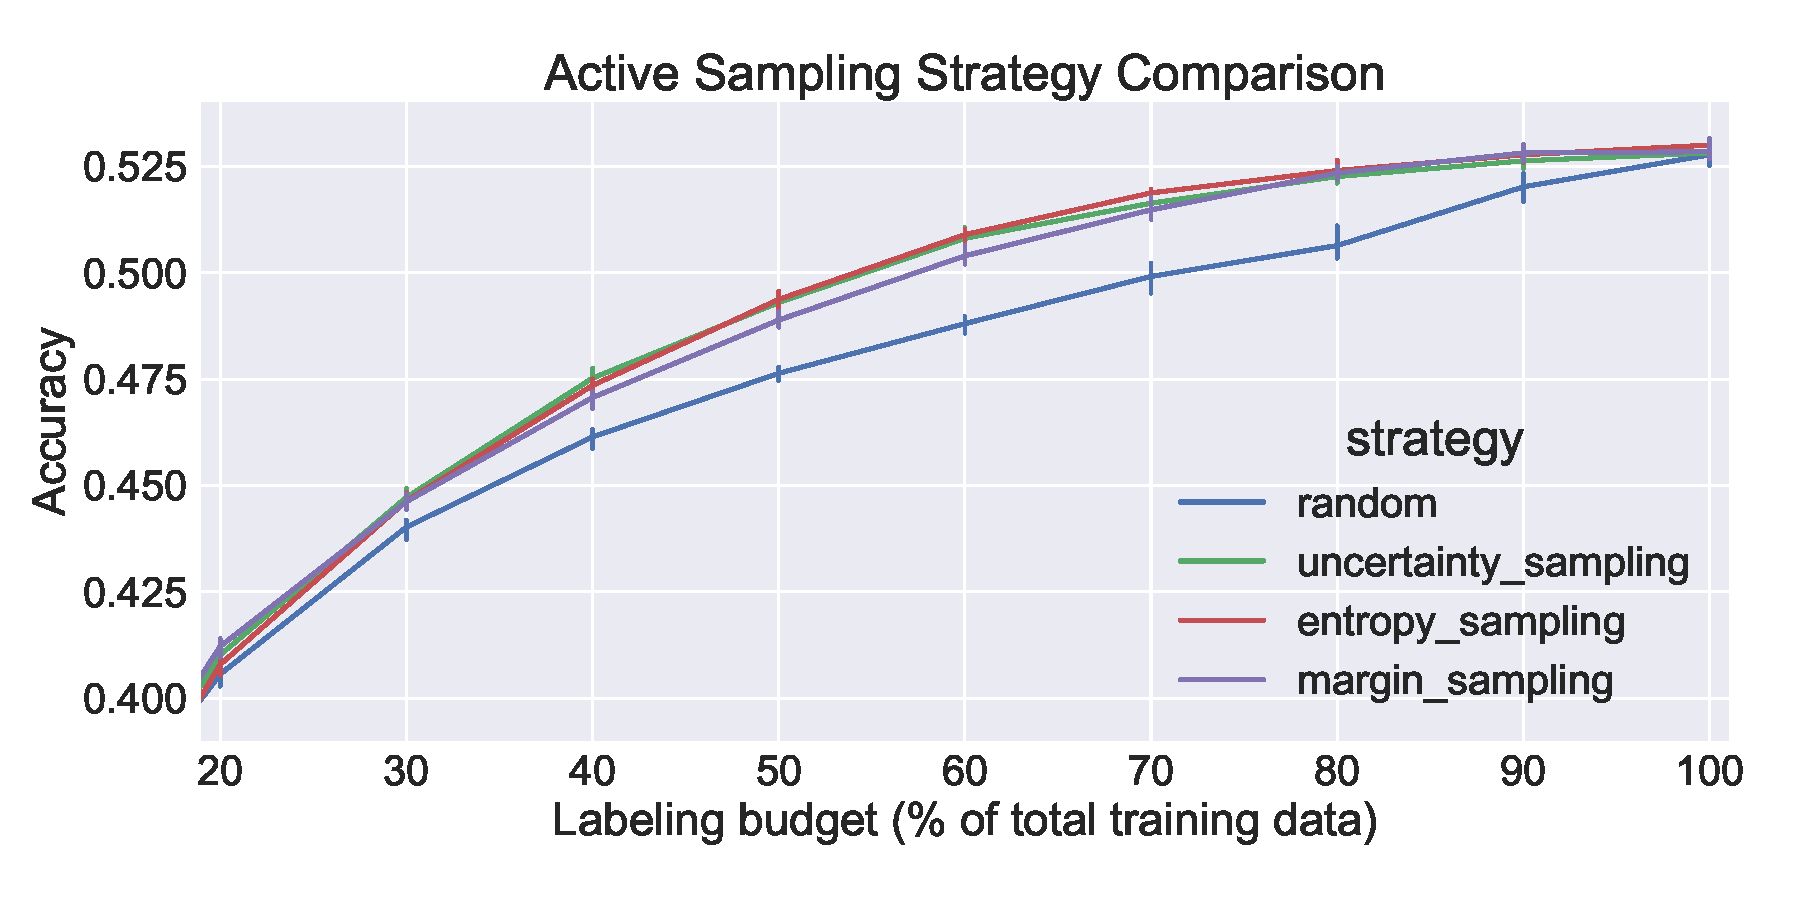
\includegraphics[width=\textwidth]{images/active_learning_manifesto.pdf} 
%
\end{center}
\caption{Comparison of active learning strategies, see \autoref{sec:active_learning_strategies}, with random baseline (blue), shown are the median and the 5th/95th percentile across 100 repetitions. While there are no distinct differences between the active learning strategies, all active learning strategies are significantly superior to randomly sampling from the pool of unlabelled data points. 
\label{fig:active_learning_curves}
}
\end{figure}

\section{Conclusion}
Our offline experiments show that active learning can be useful for speeding up annotation of political texts. The results of this study demonstrate that when using active learning can yield models that are as accurate as the best model, meaning a model trained on all available training data, with less than XX\% of the entire training data in 95\% of the experiments. Random sampling in contrast achieves only the best performance when trained on XX\% of the data. This highlights the potential of using information of the model uncertainty when deciding which samples to annotate next when the annotation budget is limited.

As we deliberately restricted the complexity of the model class to a linear classifier and simple unigram bag of words features, it is very likely that the best performing model can be improved. This does not affect the conclusion that active learning can speed up the annotation process. Our restrictions were made deliberately and merely to speed up experiments.

\subsection*{Acknowledgements}
We thank Giovanni Zappella for helpful feedback on active learning matters. We thank Jirka Lewandowski and Pola Lehmann for helpful discussions on data, modelling and support when using the public Manifesto API.
%
\small{
\bibliographystyle{plain}
\bibliography{active-manifesto} 
}


\end{document}